\documentclass{standalone}
\usepackage{pgfplots}
\pgfplotsset{soldot/.style={color=black,only marks,mark=*},
             holdot/.style={color=black,fill=white,only marks,mark=*},
             compat=1.12}
\begin{document}
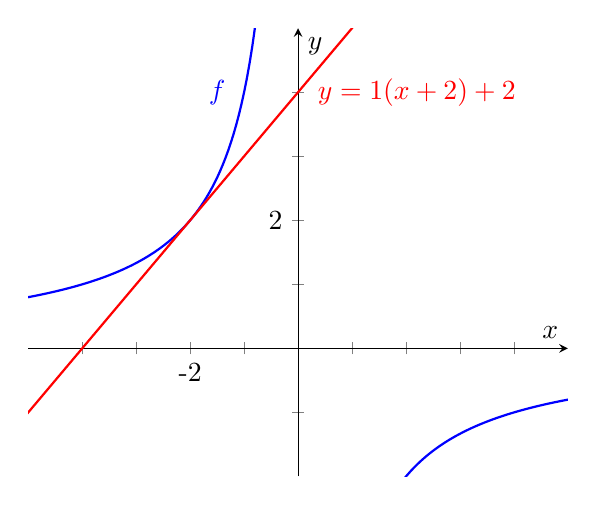
\begin{tikzpicture}
\begin{axis}[
 axis lines=middle,
 %ticklabel style={fill=blue!5!white},
 xmin=-5,xmax=5,
 ymin=-2,ymax=5,
 xtick={-4,...,1,2,3,4},xticklabels={,,-2},
 ytick={-1,...,1,2,3,4},yticklabels={,,,2},        %<--
% minor tick = {-5,-3,...,5}, %<--
 xlabel=\(x\),ylabel=\(y\),
 samples=200]

\addplot[domain=-10:-.1,thick,blue] {-4/x};
\addplot[domain=.1:10,thick,blue] {-4/x};
\addplot[domain=-10:10,thick,red] {x+4};

\draw [blue] (axis cs:-1.5,4)  node [] {$f$};
\draw [red] (axis cs:2.2,4)  node [] {$y=1(x+2)+2$};


\end{axis}
\end{tikzpicture}
\end{document}